\documentclass{beamer}
%[aspectratio=169]   \usepackage[czech]{babel}
\usepackage{apo-lecture}
\usepackage{pdfpages}
\usepackage{pdfcomment}
\usepackage{listings}
\usepackage{array,multirow}

\subtitle{Lekce 06. Superskalární architektura\\a\\prediktory skoků}
\author{Pavel Píša \phantom{xxxxxxxxx} Petr Štěpán \\ \small\texttt{pisa@fel.cvut.cz}\phantom{xxxx}\small\texttt{stepan@fel.cvut.cz}}
\begin{document}

\maketitle

\section{Superscalární architektura}

\begin{frame}
\frametitle{Cíl dnešní přednášky}

\begin{itemize}
 \item Podívat se na další možné zrychlení procesoru, které navazuje na pipelining -- superskalární architekturu
 \item Predikce skoků jako velmi důležitá vlastnost superskalárních procesorů
 \item Obě tyto techniky se využívají jak v RISC-V procesorech, tak i ve všech současných procesorech
\end{itemize}

\end{frame}

\begin{frame}[fragile]
\frametitle{Opakování - kvíz}

V kterém případě instrukce obsahují datový hazard?

\begin{columns}[T]
\begin{column}{0.40\textwidth}
\phantom{xxxxx}a)

\begin{minted}[fontsize=\footnotesize]{gas}
addi t0, s1, 4
add  t1, s1, s0
add  s1, s2, x0
\end{minted}
\end{column}
\begin{column}{0.40\textwidth}
\phantom{xxxxx}b)

\begin{minted}[fontsize=\footnotesize]{gas}
addi t0, s1, 4
add  t1, s2, s3
add  t2, t0, t1
\end{minted}
\end{column}
\end{columns}
\bigskip
\begin{itemize}
 \item[A] ani v jednom sloupci
 \item[B] hazard je pouze v případě a)
 \item[C] hazard je pouze v případě b)
 \item[D] hazard je v případě a) i b)
\end{itemize}

\end{frame}

\begin{frame}[fragile]
\frametitle{Opakování - kvíz}

Jak lze vyřešit následující datový hazard?

\begin{minted}[fontsize=\footnotesize]{gas}
lw   s2, 10(s0)
addi s1, s2, -1 
\end{minted}
\bigskip
\begin{itemize}
 \item[A] tento hazard nelze vyřešit, musí ho řešit překladač nebo programátor
 \item[B] lze ho vyřešit pomocí data forwarding
 \item[C] musí se řešit pouze pomocí stall
 \item[D] lze ho vyřešit kombinací stall a data forwarding
\end{itemize}

\end{frame}


\begin{frame}

\frametitle{Procesor s pipeline (z přednášky 5)}

Jak může Hazard Unit rozhodnout o datovém hazardu, když to dělá problémy studentům? Jednoduše:
\begin{columns}
\begin{column}{0.67\textwidth}
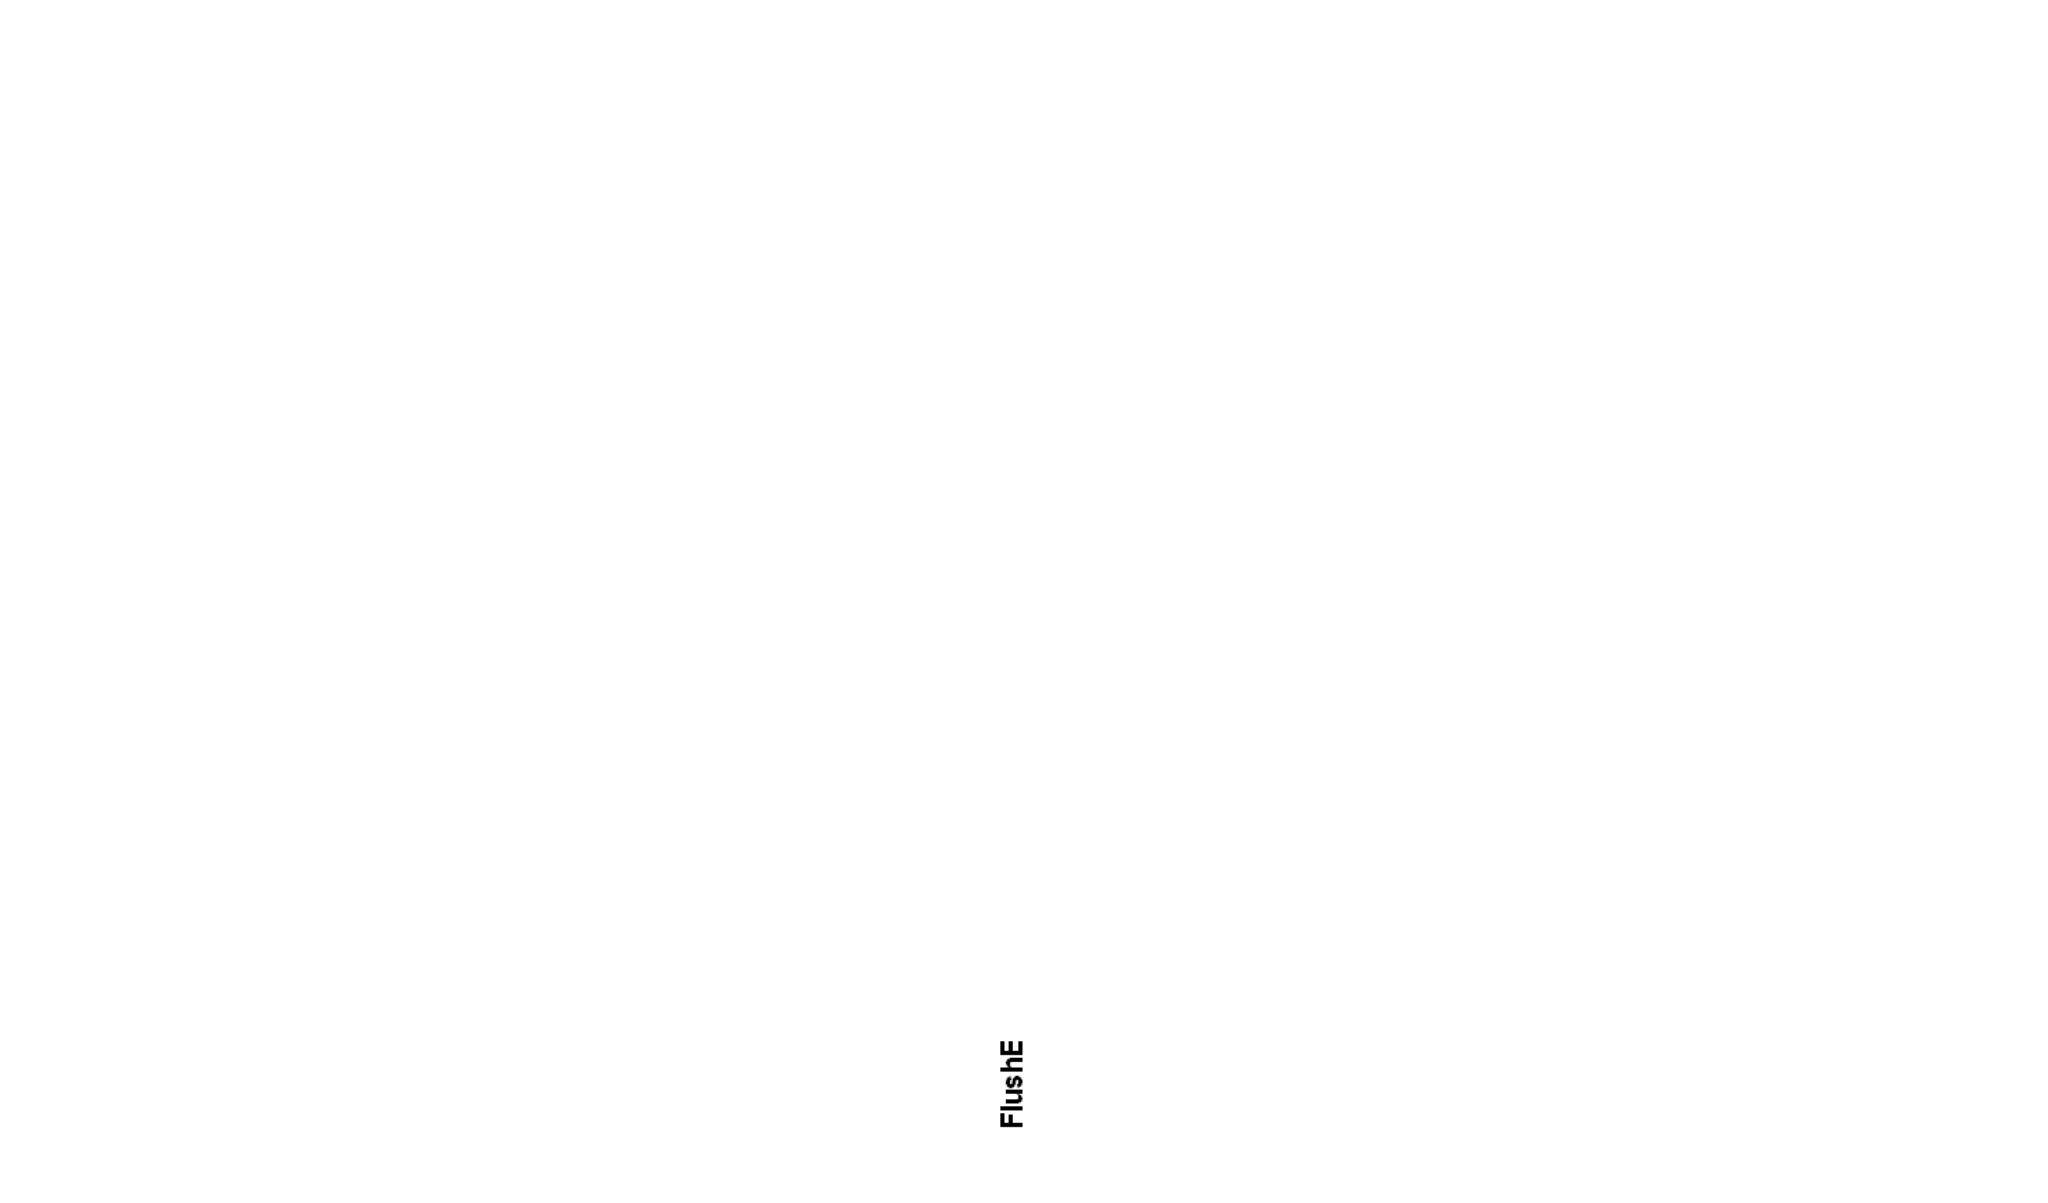
\includegraphics[width=\textwidth]{cpu_final_design.pdf}
\end{column}
\begin{column}{0.33\textwidth}
\footnotesize
\begin{itemize}
\item Pokud je RegWriteM==1, MemToRegM==0 a WriteRegM==RsE1 nebo RsE2 pak nastav ForwardAE na 2 nebo ForwardBE na 2
\item Pokud je RegWriteW==1, MemToRegW==0 a WriteRegW==RsE1 nebo RsE2 pak nastav ForwardAE na 1 nebo ForwardBE na 1
\end{itemize}
\end{column}
\end{columns}
\bigskip
\footnotesize
\begin{itemize}
\item Pokud MemToRegM==1 a WriteRegW==Rs1E nebo Rs2E pak nastav pozastavení - STALL
\end{itemize}
\end{frame}

\begin{frame}
\frametitle{Paralelismus na úrovni instrukcí}

Paralelní zpracování na úrovni instrukcí (Instruction Level Parallelism, ILP)
\begin{itemize}
 \item Pipelining -- paralelně se zpracovávají různé fáze různých instrukcí
 \item Superpipelining -- za superpipelining se označuje pipelining s více než 10 kroky. Pomalejší fáze pipeliningu se rozdělí na více částí, tím dojde k možnosti zvýšit frekvenci procesoru a tím i jeho výkon.
 \item Superskalární procesor -- paralelně se zpracovávají stejné fáze různých instrukcí
\begin{itemize}
\item můžeme mít více jednotek ALU a provádět paralelně fáze EX více různých instrukcí
\item ve fázi fetch můžeme paralelně načítat více instrukcí jdoucích po sobě, tedy např. instrukce z adresy PC, PC+4, PC+8 a PC+12
\item jednotlivé fáze instrukcí jsou navíc zřetězené, takže po paralelním načtení 4 instrukcí, rovnou načítáme další 4 instrukce 
\end{itemize}
\end{itemize}

\end{frame}

\begin{frame}
\frametitle{Paralelismus na úrovni instrukcí}

Zřetězený procesor -- piplened procesor
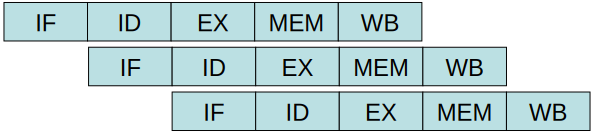
\includegraphics[width=0.85\textwidth]{pipeline.pdf}

Superskalární procesor -- super scalar procesor
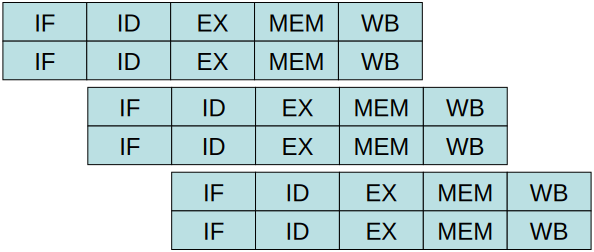
\includegraphics[width=0.85\textwidth]{superscalar.pdf}

\end{frame}

\begin{frame}
\frametitle{Superskalární procesory}

\begin{itemize}
\item Superskalární procesory mají IPC (Instruction Per Clock) větší než 1. 
  \begin{itemize}
  \item Normální i pipelined procesor mají neustále IPC=1
  \end{itemize}
\item Počet paralelních větví se nazývá šířka zřetězení (instruction pipeline width)
\item Existují dvě základní varianty:
  \begin{itemize}
  \item \textbf{Statická} superskalární architektura -- paralelně mohou být spuštěny jen instrukce jdoucí v programu za sebou.
    \begin{itemize}
    \item Pokud na sobě instrukce závisí vede to k pozastavení procesoru (stall).
    \end{itemize}
  \item \textbf{Dynamická} superskalární architektura -- paralelně mohou být spuštěny libovolné instrukce, které jsou přiravené k vykonávání. 
    \begin{itemize}
    \item Umožňuje předbíhání instrukcí tzv. out-of-order execution.
    \item Lépe využívá HW prostředky procesoru.
    \end{itemize}
  \end{itemize}
\end{itemize}

\end{frame}

\begin{frame}
\frametitle{Superskalární procesory}

\begin{itemize}
\item Jednotlivé paralelní větve mohou být \textbf{unifikované} -- tedy všechny větve jsou stejné a mohou provádět všechny typy operací
  \begin{itemize}
  \item V praxi by to byl zbytečně složitý procesor -- nepoužívá se
  \end{itemize}
\item Jednotlivé paralelní větve jsou \textbf{specializované} -- každá větev umí jen některé instrukce:
  \begin{itemize}
  \item instrukce pracující pouze s registry -- výpočty, porovnání
  \item instrukce pracující s pamětí -- načítání/ukládání dat z/do paměti
  \item instrukce skoku -- instrukce měnící PC
  \end{itemize}
\end{itemize}
\end{frame}

\section{Reorganizace výpočtů v registrech}

\begin{frame}
\frametitle{Superskalární architektura}
\begin{columns}
\begin{column}{0.55\textwidth}
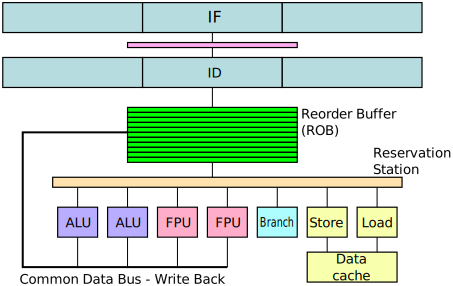
\includegraphics[width=\textwidth]{superscalar-architecture.pdf}
\end{column}
\begin{column}{0.45\textwidth}
\begin{itemize}
\item Základem architektury je ReOrder Buffer (ROB), který pomocí přejmenování registrů umí zlepšit paralelizaci instrukcí.
\item Reservation Station rozšiřuje možnosti ukládání operandů pro operace a organizuje jejich vykonávání
\item Common Data Bus zajišťuje zapsání vypočtených hodnot do skutečných registrů i pro přejmenované registry.
\end{itemize}
\end{column}
\end{columns}
\end{frame}


\begin{frame}[fragile]
\frametitle{Datové hazardy v superskalární architektuře}

Pro instrukce pracující pouze s registry:
\begin{itemize}
\item je jasné, že není možné paralelně vykonávat všechny instrukce
\item pomocí skryté sady registrů je možné paralelizaci zvýšit.
\end{itemize}

\begin{minted}[fontsize=\footnotesize]{gas}
1: slli t1, s1, 4
2: add  t0, t1, s2
3: addi s2, t0, 8
4: mult t1, s0, s0
5: addi t3, t1, 100
\end{minted}

Tento program lze paralelizovat s použitím skryté sady registrů pro přejmenování:

\begin{columns}[T]
\begin{column}{0.40\textwidth}
\begin{minted}[fontsize=\footnotesize]{gas}
1: slli RN0, s1, 4
2: add  RN1, RN0, s2
3: addi RN2, RN1, 8
\end{minted}
\end{column}
\begin{column}{0.40\textwidth}
\begin{minted}[fontsize=\footnotesize]{gas}
4: mult RN3, s0, s0
5: addi RN4, RN3, 100
\end{minted}
\end{column}
\end{columns}
\end{frame}


\begin{frame}
\frametitle{Tomasulo algoritmus}

Robert Tomasulo z IBM vymyslel v roce 1967 algoritmus pro out-of-order vykonávání výpočtů na FPU.
V současné době je jeho modifikace základem architektury všech moderních procesorů.
Základní fáze jsou:
\begin{itemize}
\item Zavedení instrukce do ROB a přejmenování registru výsledku operace - získání čísla registru ze souboru záložních registrů. 
\item Zavedení instrukce do Reservation Station a čekání na připravená data
\item Provedení výpočtu a zapsání výsledku do přejmenovaného registru přes Common Data Bus
\item Dokončení nejstarší instrukce (kruhová fronta -- FIFO) z ROB a aktualizace systémového registru.
\end{itemize}
Instrukce se mohou vypočítávat out-of-order, ale dokončení instrukcí je v pořadí programu.
\end{frame}

\begin{frame}
\frametitle{Superskalární architektura}

\begin{center}
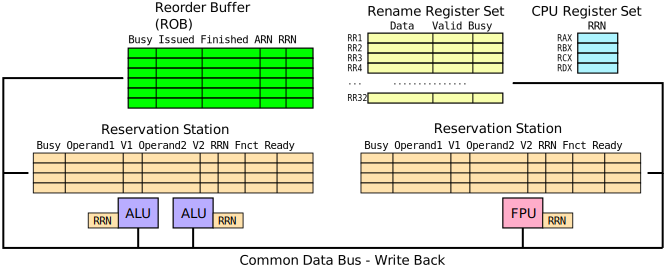
\includegraphics[width=0.7\textwidth]{superscalar-architecture2.pdf}
\end{center}

\scriptsize
Rename Register Set:
\begin{itemize}
\item Množina pomocných registrů, často i mnohokrát větší než počet CPU registrů.
\item Příznak Busy značí, že registr je využíván, Příznak valid značí, že hodnota je vypočtena a je validní. Při dokončení instrukce se nastaví CPU registr na RRN.
\end{itemize}

ReOrder Buffer:
\begin{itemize}
\item Cyklická fronta obsahuje instrukce vložené v pořadí programu
\item Fronta zaručuje, že instrukce jsou dokončovány v programovém pořadí
\item Provázání mezi Reservation Station přes číslo přejmenovaného registru (RRN Rename Register Number), který bude obsahovat výsledek operace
\item Přes Common Data Bus se dozví, že registr RRN byl vypočten a instrukce dostane příznak Finished
\item Dokončení instrukce - odstraní z ROB pouze nejstarší instrukci, až získá příznak finish.
\end{itemize}


\end{frame}

\begin{frame}
\frametitle{Superskalární architektura}

\begin{center}
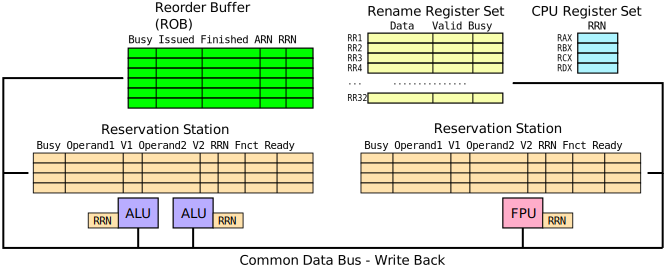
\includegraphics[width=0.7\textwidth]{superscalar-architecture2.pdf}
\end{center}

\scriptsize
Reservation Station:
\begin{itemize}
\item Obsahuje dva operandy, pokud je nastaven příznak V1/2 pak je hodnota operandu validní. Pokud není příznak V1/2 nastaven, pak operand obsahuje číslo RRN na jehož hodnotu se čeká a která přijde z CDB
\item Číslo RRN značí, do kterého registru se má zapsat výsledek.
\item Pokud jsou oba operandy validní a je volná ALU/FPU, tak se zadá provedení operace a položka se odstraní z Reservation Station (RRN výsledku se zapamatuje, aby ho ALU/FPU mohla poslat na Common Data Bus)
\end{itemize}

\end{frame}

\begin{frame}
\frametitle{Datové hazardy při čtení z paměti}

\begin{itemize}
\item Pokud instrukce lw a sw využívají jiné adresy, tak je můžeme prohazovat.
\item Pokud lw následuje po sw ze stejné adresy, lze implementovat přeposlání dat, data forwarding.
\item V praxi ale může jedna instrukce předběhnout druhou tak, že ještě není vypočteno, kam se data uloží, tedy zda dojde k hazardu.
\begin{itemize}
\item Řešení - spekulativní vykonání instrukce lw, tedy vykonání, i když není jasné, zda data budou správná
\item Při dokončování instrukce sw se zkontrolují všechny spekulativně prováděné lw 
\item Při nalezení konfliktu se zruší spekulativní provádění instrukce lw
\end{itemize}
\item Provedení se tváří, jako by bylo zachováno pořadí.
\item Velký problém v multiprocesorových systémech -- konzistence paměti při paralelních výpočtech na různých jádrech procesoru.¨
\end{itemize}

\end{frame}



\begin{frame}
\frametitle{AMD Zen2 - Mikroarchitektura}

\begin{columns}[T]
\begin{column}{0.34\textwidth}
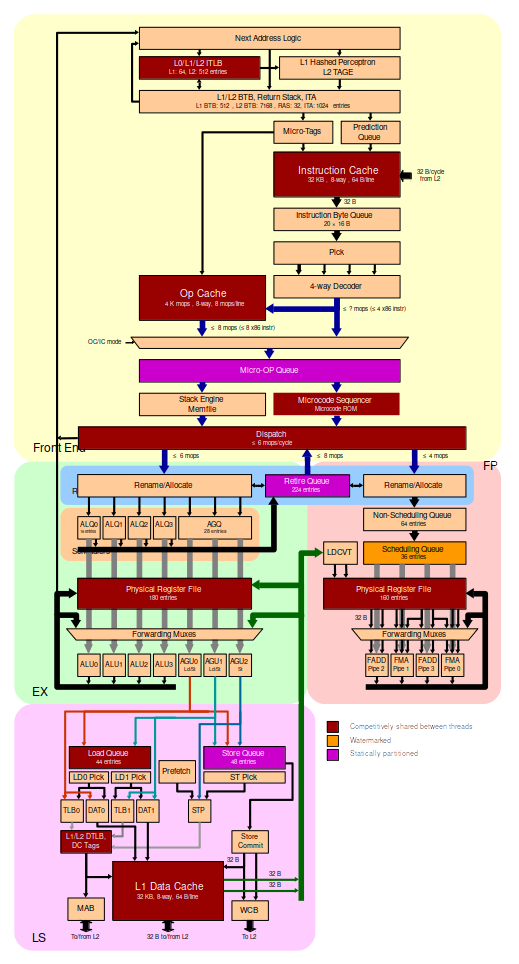
\includegraphics[width=\textwidth]{fig/amd_zen2.png}
\end{column}
\begin{column}{0.66\textwidth}
\scriptsize
\begin{itemize}
\item 7 nm process (from 12 nm), I/O die utilizes 12 nm
\item Core (8 cores on CPU chiplet),  6/8/4 µOPs in parallel
\begin{itemize}
\scriptsize
\item Frontend, µOP cache (4096 entries)
\item FPU, 256-bit Eus (256-bit FMAs) and LSU (2x256-bit L/S), 3 cycles DP vector mult latency
\item Integer, 180 registers, 3x AGU, scheduler (4x16 ALU + 1x28 AGU)
\item Reorder Buffer 224 entries
\end{itemize}
\item Memory subsystem
\begin{itemize}
\scriptsize
\item L1 i-cache and d-cache, 32 KiB each,  8-way associative
\item L2 512 KiB per core, 8-way, 
\item L2 DTLB 2048-entry
\item 48 entry store queue
\end{itemize}
\end{itemize}
Autor: QuietRub\\
Source: \url{https://en.wikichip.org/wiki/amd/microarchitectures/zen_2}
\end{column}
\end{columns}

\end{frame}


\begin{frame}
\frametitle{Opakování - kvíz}

Co je to řídicí hazard (control hazard)?

\bigskip
\begin{itemize}
 \item[A] hazard, který se musí řešit pomocí data forwarding
 \item[B] hazard, který se musí řešit pomocí stall
 \item[C] situace, kdy je nutné zahodit rozpracované instrukce
 \item[D] problém nestabilních výsledků logických operací
\end{itemize}
\end{frame}

\section{Prediktory skoku}


\begin{frame}
\frametitle{Řídicí hazardy v superskalární architektuře}

\begin{itemize}
\item Skoky v programu mění, které instrukce se vykonají.
\item Při podmíněných skocích není jasné, které instrukce se budou vykonávat.
\item Výpočet podmínky pro skok může trvat dlouho, je rozpracováno mnoho instrukcí.
\begin{itemize}
\item Řešení - spekulativní nahrání dalších instrukcí
\item Po dokončení všech výpočtů nutných pro rozhodnutí skoku se ověří, zda se mělo skákat nebo ne.
\item Při chybné predikci se musí zahodit mnoho rozpracovaných, nebo i spekulativně vykonaných instrukcí.
\end{itemize}
\item I nepodmíněné skoky mají problém, vypočítat kam se skočí. Cíl skoku může záviset na výpočtu předchozích instrukcí, a proto nejde jednoduše určit při načítání instrukcí.
\begin{itemize}
\item Řešení - spekulativně odhadneme, na jakou adresu se asi bude skákat, podle historie minulých skoků.
\item Po dokončení všech výpočtů se zkontroluje, zda se odhadla správná adresa.
\item Důležité zvláště pro návrat z funkce.
\end{itemize}
\end{itemize}

\end{frame}


\begin{frame}
\frametitle{Řídicí hazardy v superskalární architektuře}

\begin{itemize}
\item Skok je v programu statisticky každá 4 až 7 instrukce
\item 20\% skoků je nepodmíněných -- skočí se vždy, není potřeba rozhodovat
\item 80\% skoků je podmíněných
  \begin{itemize}
  \item asi 66\% je skoků na vyšší adresu, neboli dopředu 
    \begin{itemize}
    \item tyto skoky odpovídají větvení typu \texttt{if} 
    \item z nich statisticky asi 60\% se neskočí -- budeme značit \textbf{NT} (Not Taken)
    \end{itemize}
  \item zbytek asi 34\% je skoků na nižší adresu, neboli dozadu 
    \begin{itemize}
    \item tyto skoky odpovídají větvení typu \texttt{for}, \texttt{while} a \texttt{do ... while}
    \item z nich statisticky 99\% (téměř všechny) se skočí -- budeme značit \textbf{T} (Taken)
    \end{itemize}
  \end{itemize}
\end{itemize}

\end{frame}


\begin{frame}
\frametitle{Statické prediktory}

Statické prediktory mají pro danou skokovou instrukci vždy stejný výsledek:
\begin{itemize}
\item Prediktor, který by vždy odhadoval, že se vždy skočí 
\begin{itemize}
\item Podle statistiky z minulé stránky by měl úspěšnost: $p_{taken} = (0.66*0.4+0.34*0.99) = 0.60$
\item Statisticky se ukazuje, že hodnota $p_{taken}$ je pro většinu programů v rozmezí 60 -- 70\%.
\end{itemize}
\item Prediktor BTFNT -- Backwards Taken / Forwards Not Taken  
\begin{itemize}
\item Podle znaménka relativního skoku - skok zpět se skočí, skok dopředu se neskočí
\item Podle statistiky z minulého stránky by měl úspěšnost: $p_{taken} = (0.66*0.6+0.34*0.99) = 0.73$
\end{itemize}
\end{itemize}

\end{frame}

\begin{frame}[fragile]
\frametitle{Statický prediktor BTFNT}

Příklad překladu \texttt{for} cyklu:

\begin{columns}[T]
\begin{column}{0.4\textwidth}
\begin{minted}{c}
for (i=0; i<N; i++) {

  ...
  
}
\end{minted}
\end{column}
\begin{column}{0.6\textwidth}
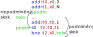
\includegraphics[width=\textwidth]{for_cyklus.pdf}
\end{column}
\end{columns}
\bigskip
Pro podmíněný skok platí, že se $N-1$ krát skočí a $1$ neskočí.\\
Skáče se vzad a pravděpodobnost správné předpovědi je tedy $\frac{N-1}{N}$

\end{frame}

\begin{frame}[fragile]
\frametitle{Statický prediktor BTFNT}

Příklad překladu \texttt{if else} konstrukce:

\begin{columns}[T]
\begin{column}{0.4\textwidth}
\begin{minted}{c}
if (a<b) {
  
  ...

} else {

  ...

}
\end{minted}
\end{column}
\begin{column}{0.6\textwidth}
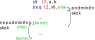
\includegraphics[width=\textwidth]{if_preklad.pdf}
\end{column}
\end{columns}
\bigskip
Nepodmíněný skok závisí na hodnotách a, b, nelze tedy o něm obecně nic prohlásit, jedině skáče se vždy dopředu.\\
Statistické chování záleží na typu programu, ale pro směs různých programů se ukazuje, že pravděpodobnost skoku je $0.4$.

\end{frame}


\begin{frame}
\frametitle{Dynamické prediktory}

\small
Dynamické prediktory se snaží odhadnout, zda se skočí na základě minulého chování dané instrukce skoku:
\begin{itemize}
\item Bylo by ideální, aby každá instrukce skoku měla svůj prediktor
\begin{itemize}
\small
\item To ale není možné, skoková instrukce může být na kterémkoliv místě paměti 4GiB
\end{itemize}
\end{itemize}


\begin{columns}[T]
\begin{column}{0.5\textwidth}
\small
Řešení: budeme mít $2^k$ prediktorů a podle $k$ nejnižších bitů adresy instrukce skoku vybereme prediktor
\begin{itemize}
\item Některé instrukce skoku na rozdílných adresách, ale se stejnými nejnižšími $k$ bity adresy se budou ovlivňovat -- \textbf{interferovat}.
\item Interference mohou velmi nepříznivě ovlivnit úspěšnost predikce.
\end{itemize}
\end{column}
\begin{column}{0.5\textwidth}
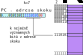
\includegraphics[width=\textwidth]{prediction_table.pdf}
\end{column}
\end{columns}

\end{frame}


\begin{frame}
\frametitle{1-bitový Smithův prediktor}

Nejjednodušší prediktor je 1-bitový Smithův prediktor
\begin{itemize}
\item Má pouze dva stavy, přepíná se podle minulého chování
\item Předpovídá, že to dopadne, jak to dopadlo minule.
\begin{itemize}
\item velmi jednoduchá implementace, vyhodnocení i úprava podle skutečnosti
\end{itemize}
\end{itemize}

\begin{center}
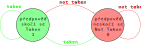
\includegraphics[width=0.45\textwidth]{smith_1bit.pdf}
\end{center}

\end{frame}

\begin{frame}[fragile]
\frametitle{1-bitový Smithův prediktor}

Predikce pro for cyklus:

\begin{columns}[T]
\begin{column}{0.35\textwidth}
\begin{minted}{c}
for (i=0; i<5; i++) {
  ...
}
\end{minted}
\end{column}
\hfill
\begin{column}{0.45\textwidth}
\begin{minted}{gas}
      addi t0, x0, 0
      addi t1, x0, 5
      j podm
telo: ...
      addi t0, t0, 1
podm: slt  t2, t0, t1
      bne  t2, x0, telo
\end{minted}
\end{column}
\end{columns}
\bigskip
Pokud prediktor neinterferuje s jinými skoky, pak začíná ve stavu 0 -- NT (Not taken).

\begin{tabular}{|l|c|c|c|c|c|c|}\hline
Skutečné chování & T & T & T & T & T & NT\\ \hline
Predikce         & {\color{red}NT} & T & T & T & T & {\color{red}T}\\ \hline
\end{tabular}

Vidíte, že prediktor není úspěšný na počátku for cyklu a na jeho konci.

Úspěšnost 1-bitového Smithova prediktoru pro cyklus s $r$ iteracemi je $\frac{r-2}{r}$.
\end{frame}


\begin{frame}
\frametitle{2-bitový Smithův prediktor}

2-bitový Smithův prediktor patří stále k těm nejjednodušším
\begin{itemize}
\item Má již 4 stavy, reprezentované dvěma bity.
\item 2 stavy předpovídají skok, 2 stavy předpovídají neskočení
\item Předpověď závisí na minulém chování, ale toleruje jednu odchylku od pravidelnosti
\item Velmi jednoduchá implementace, vyhodnocení i úprava podle skutečnosti
\end{itemize}

\begin{center}
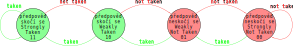
\includegraphics[width=0.95\textwidth]{smith_2bit.pdf}
\end{center}
\end{frame}

\begin{frame}[fragile]
\frametitle{2-bitový Smithův prediktor}

Predikce pro for cyklus:

\begin{columns}[T]
\begin{column}{0.35\textwidth}
\begin{minted}{c}
for (i=0; i<5; i++) {
  ...
}
\end{minted}
\end{column}
\hfill
\begin{column}{0.45\textwidth}
\begin{minted}{gas}
      addi t0, x0, 0
      addi t1, x0, 5
      j podm
telo: ...
      addi t0, t0, 1
podm: slt  t2, t0, t1
      bne  t2, x0, telo
\end{minted}
\end{column}
\end{columns}
\bigskip
\small
Pokud prediktor neinterferuje s jinými skoky, pak začíná ve stavu 10 -- WT (Weakly taken).

\begin{tabular}{|l|c|c|c|c|c|c|c|}\hline
Skutečné chování & T & T & T & T & T & NT &\\ \hline
Stav & WT & ST & ST & ST & ST & ST & WT\\ \hline
Predikce         & T & T & T & T & T & {\color{red}T} &\\ \hline
\end{tabular}

Vidíte, že prediktor není úspěšný pouze na konci for cyklu.

Úspěšnost 2-bitového Smithova prediktoru pro cyklus s $r$ iteracemi je $\frac{r-1}{r}$.
\end{frame}


\begin{frame}
\frametitle{2-bitový Smithův prediktor s hysterezí}

Obdoba 2-bitového Smithova prediktoru
\begin{itemize}
\item Při dvou změnách po sobě se přejde rovnou do stavu Strongly a musí přijít další dvě opačné chování po sobě aby se prediktor překlopil do nového stavu.
\end{itemize}

\begin{center}
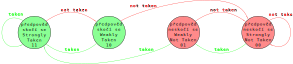
\includegraphics[width=0.95\textwidth]{smith_2bit_hist.pdf}
\end{center}
\end{frame}


\begin{frame}
\frametitle{Hodnocení prediktorů}

\begin{itemize}
\item Je nemožné rozhodnout obecně, kdy je který prediktor lepší. Vždy lze najít protipříklady, kdy je každý z uvedených prediktorů chová nejlépe
\item Jediná možnost je statistická analýza různých programů:
\end{itemize}
\begin{center}
\begin{tabular}{|l|c|} \hline
Statický prediktor - vždy se skočí & 59.25 \\\hline
1-bitový Smithův prediktor         & 68.75 \\\hline
2-bitový Smithův prediktor s hysterezí & 81.75 \\\hline
\end{tabular}
\end{center}

Zdroj: \url{https://ieeexplore.ieee.org/document/6918861}\\
H. Arora, S. Kotecha and R. Samyal, "Dynamic Branch Prediction Modeller for RISC Architecture," 2013 International Conference on Machine Intelligence and Research Advancement, Katra, 2013, pp. 397-401.
\end{frame}

\begin{frame}[fragile]
\frametitle{Závislost předpovědi}

V praxi se ukazuje, že predikce závisí na předchozím chování program.

\begin{minted}{c}
if (x==2) {  // skok s1
}
if (y==2) { // skok s2
}
if (x!=y) { // skok s3
}
\end{minted}

Pokud se proměnné \texttt{x}, \texttt{y} nemění v tělech podmínek \texttt{s1} a \texttt{s2}, pak tady máme silnou závislost skoku \texttt{s3}:

\bigskip

\begin{tabular}{|l|l|l|l|}\hline
s1 & s2 & $\implies$ s3 & vysvětlení \\\hline
neskočí & skočí   & neskočí & x==2 a y!=2 tedy platí x!=y \\\hline
skočí   & neskočí & neskočí & x!=2 a y==2 tedy platí x!=y \\\hline
neskočí & neskočí & skočí   & x==2 a y==2 tedy neplatí x!=y\\\hline 
skočí   & skočí   & nevíme  & x!=2 a y!=2 nevíme zda platí x!=y \\\hline
\end{tabular}
\end{frame}



\begin{frame}
\frametitle{Historie skoků -- korelované prediktory}

Registr BHR (Branch Histrory Register) obsahuje informaci, zda posledních $m$ skoků provedlo skok:
\begin{itemize}
\item Pokud se skočilo pak obsahuje 1, pokud se neskočilo pak obsahuje 0
\item Nová informace se vloží na nejnižší bit, nejstarší informace se vyhodí z nejvyšší pozice, ostatní informace se posune.
\end{itemize}

\begin{columns}[T]
\begin{column}{0.5\textwidth}
\small
Pro zjištení indexu prediktoru se vezme $k-m$ nejnižších bitů adresy instrukce skoku a tato informace se spojí s bity z BHR
\begin{itemize}
\item Výhoda -- podle předchozích skoků se vybere jiný prediktor.
\item Nevýhoda -- některé kombinace se v BHR nevyskytnou, a proto se tyto prediktory nepoužijí.
\end{itemize}
\end{column}
\begin{column}{0.5\textwidth}
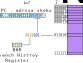
\includegraphics[width=\textwidth]{prediction_BHR.pdf}
\end{column}
\end{columns}

\end{frame}

\begin{frame}
\frametitle{GShare prediktory}

GShare přístup je podobný předchozímu:
\begin{itemize}
\item Také využívá BHR registr, který v této implementaci má přímo $k$ bitů
\end{itemize}

\begin{columns}[T]
\begin{column}{0.5\textwidth}
\small
Pro zjištení indexu prediktoru se vezme $k$ nejnižších bitů adresy instrukce skoku a provede se xor s bity z BHR.

Výhody:
\begin{itemize}
\item lépe statisticky pokryje všechny prediktory.
\item umožňuje použít delší BHR registr.
\end{itemize}
\end{column}
\begin{column}{0.5\textwidth}
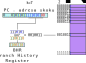
\includegraphics[width=\textwidth]{prediction_GShare.pdf}
\end{column}
\end{columns}
\end{frame}


\begin{frame}
\frametitle{Turnajové prediktory}

Základem turnajového prediktoru je soutěž dvou jiných, jednodušších prediktorů. Pro výběr, který prediktor je lepší a tedy, který prediktor bude na výstupu, lze použít 1-bitový, nebo 2-bitový prediktor. 

\bigskip
Jak funguje 1-bitový turnajový prediktor
\begin{itemize}
\item Vypočti predikci prediktory P1 a P2.
\item Pokud se predikce shodují je výsledkem tato predikce.
\item Pokud se predikce neshodují:
\begin{itemize}
\item Výsledná predikce je podle toho, který prediktor byl v minulosti úspěšný. Tato informace je uložena v 1-bitovém stavovém automatu. 
\item Podle skutečnosti vyber prediktor P1, nebo P2 pro příští predikci.
\end{itemize}
\end{itemize}
\end{frame}

\begin{frame}
\frametitle{Turnajové prediktory}

\begin{center}
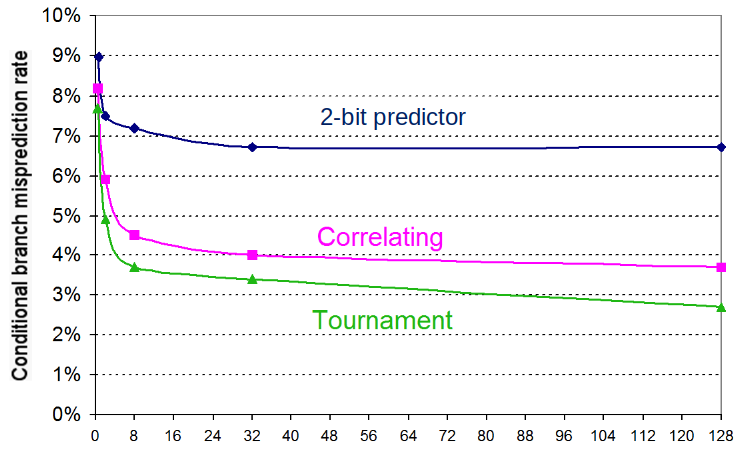
\includegraphics[width=0.75\textwidth]{fig/tournament.png}\\
\small Velikost prediktorů v KiB
\end{center}
\end{frame}

\begin{frame}
\frametitle{Opakování - kvíz}

Který prediktor nejlépe zvládne predikovat následující skutečnost skoků pokud začíná ve stavu Taken, nebo Weakly Taken:

\begin{tabular}{|c|c|c|c|c|c|c|c|c|}\hline
T & T & T & NT & NT & NT& T & T & T \\ \hline
\end{tabular}

\bigskip
\begin{itemize}
 \item[A] 1-bitový Smithův prediktor
 \item[B] 2-bitový Smithův prediktor
 \item[C] 2-bitový Smithův prediktor s hysterezí
 \item[D] všechny udělají stejný počet chyb
\end{itemize}
\end{frame}


\begin{frame}
\frametitle{Perceptron}

\begin{center}
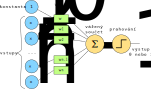
\includegraphics[width=0.6\textwidth]{neuron.pdf}
\end{center}

Pro výpočet hodnoty se použije vzoreček $\xi = \sum_{i=0}^{n} x_i \cdot w_i$. Závěrečné vyhodnocení je pomocí přenosové funkce, v našem případě skokové funkce, která má tvar:
$f(\xi) = \begin{cases}1& \text{pro } \xi \ge 0\\0& \text{pro }\xi <0\end{cases}$ 
\end{frame}


\begin{frame}
\frametitle{AMD Zen2 prediktor}

\begin{center}
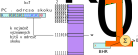
\includegraphics[width=0.7\textwidth]{prediction_amd.pdf}
\end{center}

Podle adresy skoku se vybere jeden perceptron z tabulky. 

Perceptron je definován vahami $w_i$. 

Výsledek predikce je znaménko váženého součtu $\xi = \sum_{i=0}^{n} x_i \cdot w_i$, kde $x_i$ jsou bity z registru historie skoků BHR.

Výhoda -- lepší výsledky než gshare, lze použít i pro dlouhé registry historie BHR, nevýhoda -- složitý výpočet, nelze získat výsledek v jednom taktu procesoru.
\end{frame}

\begin{frame}
\frametitle{AMD Zen2 -- Predikce skok}

\begin{itemize}
\item Výpočet výstupu perceptronu je relativně pomalý, normální perceptrony používají reálná čísla s plovoucí desetinnou čárkou. Je možné urychlit 16-ti bitovými reálnými čísly, nebo použitím pevné desetinné čárky.
\item Skutečná implementace prediktorů skoků má tři úrovně
\begin{itemize}
\item úroveň 1 -- 16 velmi rychlých prediktorů, rozhodnou ještě v tom samém hodinovém cyklu, které další instrukce načítat
\item úroveň 2 -- 512 prediktorů, které v dalším hodinovém cyklu upřesní předpověď, buď se zahodí načítané instrukce, nebo se potvrdí
\item úroveň 3 -- 7168 prediktorů, za 4 hodinové cykly zpřesní předpověď. Opět se dosavadní načtené instrukce buď uchovají, nebo zahodí.
\end{itemize}
\item Průměrná časová prodleva při špatné konečné predikci je přibližně 18 hodinových cyklů.
\item Při rychlosti 4GHz a pokud je každá desátá instrukce skok, tak 1\% chybné predikce vede ke snížení výkonu o téměř 2\%.
\end{itemize}
\end{frame}


\begin{frame}
\frametitle{AMD Zen2 prediktor}

\begin{center}
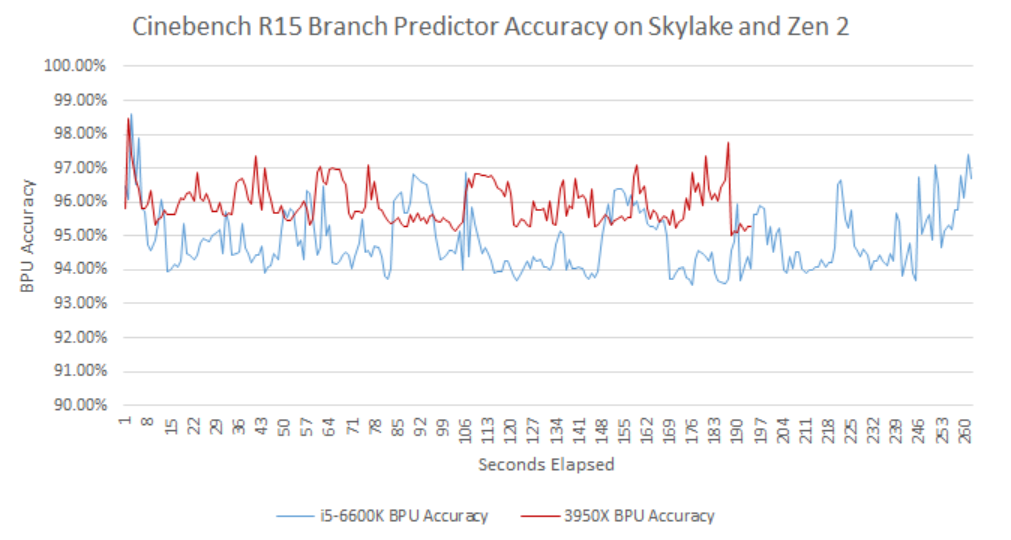
\includegraphics[width=0.8\textwidth]{fig/amd_cinebench.png}
\end{center}

Zdroj: Analyzing Zen 2’s Cinebench R15 Lead
By clamchowder from \url{https://chipsandcheese.com}
\end{frame}

\section{Predikce cíle skoku}

\begin{frame}
\frametitle{Predikce cíle skoku}

Skoky mají jak v RISC-V tak v ostatních procesorech různý formát cílové adresy skoku:
\begin{itemize}
\item skok na pevnou adresu -- cíl skoku je adresa přímo uvedená v instrukci skoku (není v RISC-V, protože má pevnou délku instrukce a 32-bitová adresa se do kódu instrukce nevejde)
\item skok relativně vůči adrese skokové instrukce -- cíl skoku se vypočte jako součet PC v okamžiku načtení skokové instrukce a zadaná konkrétní hodnota v instrukci.
\item skok na pozici uvedenou v registru, nebo v paměti -- RISC-V má instrukci \texttt{jalr}, tedy skok na adresu uvedenou v registru, x86 obsahuje instrukce \texttt{ret} -- návrat z podprogramu podle adresy uvedené v paměti na zásobníku a instrukci \texttt{jump indirect}, kdy adresa ukazuje do paměti, kde je uvedena cílová adresa skoku (tuto instrukci lze použít při skoku podle tabulky např. při překladu \texttt{switch} konstrukce, nebo při volání funkcí dynamických knihoven). 
\end{itemize}
\end{frame}

\begin{frame}
\frametitle{Predikce cíle skoku}

\begin{itemize}
\item Cíl skoku je potřeba zjistit již ve fázi načítání instrukcí.
\item Lze mít speciálně dedikované sčítačky na cílové adresy skoku, ale i tam součet nějakou dobu trvá.
\item Proto je důležité odhadnout cíl skoku:
\begin{itemize}
\item BTB (Branch Target Buffer) je buď plně asociativní paměť nebo částečně
asociativní s daným stupněm asociativity
\item Řádky jsou dvojice: 
\begin{itemize}
\item klíč -- BIA (Branch Instruction Address) -- tedy hodnota PC v okamžiku skoku
\item BTA (Branch Target Address) -- cílová adresa skoku
\end{itemize}
\end{itemize}
\item Pokud se PC shoduje s hodnotou BIA v BTB a současně prediktor předpoví, že se skočí, změní se PC spekulativně na hodnotu příslušné BTA
\end{itemize}
\end{frame}

\begin{frame}
\frametitle{Predikce návratu z funkce}

Nejčastější skok podle adresy v paměti je návrat z funkce:
\begin{itemize}
\item Pro rychlou predikci adresy návratu z funkce obsahují moderní CPU -- Return Address Stack (RAS)
\begin{itemize}
\item Jedná se o rychlou paměť typu zásobník -- pamatující si omezené množství (až 32) návratových adres
\item Hodnota se do RAS uloží při volání funkce, při načtení instrukce ret pak vrchol RAS slouží jako prediktor cíle skoku
\end{itemize}
\item Funguje spolehlivě pro úrovně vnoření funkcí podle velikosti RAS
\end{itemize}
\end{frame}

\section{Odstranění skoků z programu}

\begin{frame}[fragile]
\frametitle{Ukázka, jak odstranit skok v programu}

Na internetu můžete najít mnoho triků, jak odstranit podmínku a tedy podmíněný skok ve Vašich programech.

Zde si ukážeme odstranění if z výpočtu absolutní hodnoty celého čísla:

\begin{columns}[T]
\begin{column}{0.01\textwidth}
\phantom{x}
\end{column}
\begin{column}{0.25\textwidth}
program v C
\begin{minted}[fontsize=\small]{c}
if (x<0) {
  x = -x;
}
\end{minted}
\end{column}

\begin{column}{0.28\textwidth}
program v RISC-V
\begin{minted}[fontsize=\small]{gas}
 slt t0, s0, x0
 beq t0, x0, skip
 sub s0, x0, s0
skip:
\end{minted}
\end{column}
\begin{column}{0.45\textwidth}
\phantom{x}komentář\\
\small
porovná, zda x<0\\
podle výsledku skočí, nebo ne\\
vypočte -x
\end{column}
\end{columns}
\bigskip

Odstranit podmíněný skok, který by se velmi špatně odhadoval lze následující konstrukcí, využívající nejvyšší znaménkový bit:
\begin{columns}[T]
\begin{column}{0.01\textwidth}
\phantom{x}
\end{column}
\begin{column}{0.25\textwidth}
program v C
\begin{minted}[fontsize=\small]{c}
int tmp = x>>31;
x ^= tmp;
x -= tmp;
\end{minted}
\end{column}

\begin{column}{0.28\textwidth}
program v RISC-V
\begin{minted}[fontsize=\small]{gas}
srai t0, s0, 31
xor  s0, s0, t0
sub  s0, s0, t0
\end{minted}
\end{column}
\begin{column}{0.45\textwidth}
\phantom{x}komentář\\
\small
tmp bude buď 0, nebo 0xFFFFFFFF\\
nedělá nic, nebo bitovou inverzi\\
pro tmp==0 nedělá nic, jinak odečte -1, tedy přičte 1
\end{column}
\end{columns}
\end{frame}

\begin{frame}[fragile]
\frametitle{Ukázka, jak odstranit skok v programu}

Pokud je hodnota b rovna 0, nebo 1, pak lze následující C program:

\begin{minted}[fontsize=\small]{c}
a = ( (b!=0) ? c : d);
\end{minted}

změnit na program:

\begin{minted}[fontsize=\small]{c}
static const int lookup_table[] = {d,c};
a = lookup_table[b];
\end{minted}

\bigskip
Odstranit lze i více skoků najednou, pokud opět b1, b2, b3 budou nabývat pouze hodnot 0, nebo 1:

\begin{minted}[fontsize=\small]{c}
a = ( b1 ? c : ( b2 ? d : (b3 ? e : f)));
\end{minted}

lze změnit na program:

\begin{minted}[fontsize=\small]{c}
static const int lookup_table[] = { f, e, d, d, c, c, c, c };
a = lookup_table[b1 * 4 + b2 * 2 + b3];
\end{minted}
\end{frame}

\begin{frame}[fragile]
\frametitle{Ukázka, jak odstranit skok v programu}

Obdobně převod čísla od 0 do 15 na hex znak lze buď
\begin{minted}[fontsize=\small]{c}
if (a<10) {
  ch = '0'+a;
} else {
  ch = 'A'+(a-10);
}
\end{minted}

lze změnit na program:

\begin{minted}[fontsize=\small]{c}
static const int hex_c[] = {'0','1','2','3','4','5','6','7',
                            '8','9','A','B','C','D','E','F'};
ch = hex_c[a];
\end{minted}
\end{frame}

\end{document}

